\documentclass[twoside,letterpaper,openany]{book}

%\usepackage{geometry}                % See geometry.pdf to learn the layout options. There are lots.
%\geometry{letterpaper}                   % ... or a4paper or a5paper or ... 
%\geometry{landscape}                % Activate for for rotated page geometry
%\usepackage[parfill]{parskip}    % Activate to begin paragraphs with an empty line rather than an indent
%\usepackage{graphicx}
%\usepackage{epstopdf}
%\DeclareGraphicsRule{.tif}{png}{.png}{`convert #1 `dirname #1`/`basename #1 .tif`.png}
%\usepackage{amsthm}

\usepackage[top=1in,left=1in,right=1in,bindingoffset=5mm,twoside]{geometry}

\usepackage{amssymb}
\usepackage{amsmath}
\usepackage{enumitem}
\usepackage{framed}
\usepackage[framed]{ntheorem}
\usepackage{dsfont}
\usepackage{bm}
\usepackage{quoting}
\usepackage{setspace}
\usepackage{xifthen}
\usepackage{textcomp}
\usepackage{nameref}
\usepackage{tikz}
\usepackage{graphicx}




\newcommand\onestar{$\star$}
\newcommand\twostar{$\star\star$}
\newcommand\threestar{$\star\star\star$}



\theoremstyle{margin}
\theorembodyfont{\normalfont}
\theoremseparator{.}
\theorempreskipamount=\baselineskip
\theorempostskipamount=-1.5em

\theoremprework{\begin{onehalfspace}} \theorempostwork{\end{onehalfspace}}
\newtheorem{defn}{Definition}  %[chapter]

\theoremprework{\begin{onehalfspace}} \theorempostwork{\end{onehalfspace}}
\newtheorem{example}[defn]{Example}

\theoremprework{\begin{onehalfspace}} \theorempostwork{\end{onehalfspace}}
\newtheorem{axiom}[defn]{Axiom}

\newtheorem{corol}[defn]{Corollary}

\newtheorem{conjecture}[defn]{Conjecture}


\theoremprework{\begin{onehalfspace}} \theorempostwork{\end{onehalfspace}}
\newtheorem{thmex}[defn]{Example Theorem}

\theoremheaderfont{\scshape}
\theoremindent\parindent
\newtheorem*{proofex}[defn]{Example Proof}
\theoremheaderfont{\normalfont\bfseries}
\theoremindent0cm

\theoremstyle{plain}
\theorembodyfont{\normalfont}
%\theoremindent=\parindent
%\theoremseparator{.}

\theorempreskipamount=-2em
\theorempostskipamount=-.75em

\newframedtheorem{thm}[defn]{Theorem}

\newframedtheorem{thm1}[defn]{\raisebox{.1em}{\onestar} Theorem}
\newframedtheorem{thm2}[defn]{\raisebox{.1em}{\twostar} Theorem}
\newframedtheorem{thm3}[defn]{\raisebox{.1em}{\threestar} Theorem}


\newframedtheorem{lemma}[defn]{Lemma}
\newframedtheorem{lemma1}[defn]{\raisebox{.1em}{\onestar} Lemma}
\newframedtheorem{lemma2}[defn]{\raisebox{.1em}{\twostar} Lemma}
\newframedtheorem{lemma3}[defn]{\raisebox{.1em}{\threestar} Lemma}

\newcommand\stmtword{Proposition}
\newframedtheorem{stmt}[defn]{\stmtword}

\newframedtheorem{stmt1}[defn]{\raisebox{.1em}{\onestar} \stmtword}
\newframedtheorem{stmt2}[defn]{\raisebox{.1em}{\twostar} \stmtword}
\newframedtheorem{stmt3}[defn]{\raisebox{.1em}{\threestar} \stmtword}


\newframedtheorem{exer}[defn]{Exercise}

\newframedtheorem{exer1}[defn]{\raisebox{.1em}{\onestar} Exercise}

\newframedtheorem{exer2}[defn]{\raisebox{.1em}{\twostar} Exercise}

\newframedtheorem{exer3}[defn]{\raisebox{.1em}{\threestar} Exercise}


\newframedtheorem{progexer}[defn]{Programming Exercise}


\newenvironment{exersoln}[1]{\textbf{Exercise #1 Solution.}\begin{quote}}{\end{quote}}
\newenvironment{stmtsoln}[1]{\textbf{\stmtword\ #1 Proof.}\begin{quote}}{\end{quote}}
\newenvironment{thmsoln}[1]{\textbf{Theorem #1 Proof.}\begin{quote}}{\end{quote}}
\newcommand\answer{\par\textbf{\emph{Answer}.\ }}
\newcommand\proof{\par\textbf{\emph{Proof}.\ }}

\newenvironment{exenumerate}{\begin{enumerate}[label=(\alph*),leftmargin=3em]}{\end{enumerate}}
%\newenvironment{discussion}{\begin{quoting}[vskip=0pt]}{\end{quoting}}
\newenvironment{discussion}{\begin{leftbar}\noindent}{\end{leftbar}}
%\newenvironment{discussion}{}{}

\newcommand\defterm[1]{\emph{\textbf{#1}}}  % a term being defined
\newcommand\hint{\\ \emph{Hint:}\ }
\newcommand*{\happymac}{\hfill
\includegraphics[height=2em]{happymac.png}\\}

\newcommand\emptystring\epsilon
\newcommand\definedas{\ \equiv\ }
%\newcommand\implies\to
\newcommand*{\qed}{\hfill\ensuremath{\square}}

\newcommand\naturals{\mathds{N}}

\newcommand\setbuildsepname{colon}
\newcommand\setbuildsep{:}
\newcommand\setdef[1]{\left\lbrace #1 \right\rbrace}
\newcommand\setbuild[2]{\left\lbrace #1\ \setbuildsep\ #2 \right\rbrace}
\newcommand\union\cup
\newcommand\intersection\cap
\newcommand\setunion[2]{#1\,\union\,#2}
\newcommand\setintersection[2]{#1\,\intersection\,#2}
\newcommand\setconcat[2]{#1\,\circ\,#2}
\newcommand\setcomplement[1]{\overline{#1}}
\newcommand\setstar[1]{#1^{*}}
\newcommand\powerset[1]{\mathcal{P}(#1)}
\newcommand\setproduct[2]{#1 \times #2}
\newcommand\yields{\ \Rightarrow\ }
\newcommand\derives{\ \Rightarrow^*\ }

\newcommand\langof[1]{\mathcal{L}(#1)}

\newcommand\stringrev[1]{#1^{\mathcal{R}}}


\title{Theory of Computation \\ \vspace{2mm} {\large Course Notes}}
\author{Nadeem Abdul Hamid}
\date{\today}

%%%%%%%%%%%%%%%%%%%%%%%%%%%%%%
\begin{document}

\maketitle

%%%%%%%%%%%%%%%%%%%%%%%%%%%%%%
\chapter*{Preface}


%%%%%%%%%%%%%%%%%%%%%%%%%%%%%%
\setcounter{secnumdepth}{0}
\tableofcontents

\newpage
\section{List of axioms, definitions, and proved theorems}
\listtheorems{axiom,defn,thmex}

%%%%%%%%%%%%%%%%%%%%%%%%%%%%%%
\setcounter{chapter}{-1}
\chapter{Introduction}\label{chapter:intro}
	\section{Warm-up}

\begin{discussion}
Central to the study of the theory of computation are the concepts of ``alphabet'' (a set of symbols), ``string'' (a list of symbols from an alphabet), and ``language'' (a set of strings from the same alphabet). In this section, we will work through some simple, intuitive definitions of these concepts. In the chapter that follows, we will review some formal mathematical notation (that should be familiar from a discrete structures course) and then provide more precise definitions of some concepts presented here.
\end{discussion}

\begin{defn}[Alphabet]
An \defterm{alphabet} is a finite set of \defterm{symbols}. We'll often use $\Sigma$ (``uppercase sigma") for an alphabet.
\end{defn}

\begin{defn}[String]
A \defterm{string over an alphabet} (sometimes called a \defterm{word}) is a finite sequence of symbols from the alphabet. We generally use $u, v, w, x, y, z$, and lowercase Greek letters to denote strings. 
\end{defn}

\begin{defn}[Empty string]
The string with no symbols at all, called the \defterm{empty string}, is denoted by $\bm\emptystring$.
\end{defn}

\begin{defn}[$\Sigma^*$]
The set of all strings, including the empty string, over an alphabet $\Sigma$ is denoted by $\bm{\Sigma^*}$.
\end{defn}

\begin{exer}
List at least 10 strings that are in the set $\setstar{\setdef{0, 1}}$. 
\end{exer}

\begin{defn}[String length]
The \defterm{length} of a string is the number of symbols it contains. We denote the length of a string $w$ by $|w|$. If $w$ has length $n$, we can write $w = w_1 w_2 \,\cdots\, w_n$ where each symbol $w_i \in \Sigma$. 
\end{defn}

\begin{exer}
What is $|\emptystring|$?
\end{exer}

\begin{defn}[String concatenation]
The \defterm{concatenation} of two strings $x$ and $y$, written $xy$, is the string $x$ followed by the string $y$. To concatenate a string with itself many times, we use the superscript notation $x^k$ to mean:
\[\overbrace{x\,x\,\cdots\,x}^k\]
\end{defn}

\begin{defn}[String reverse]
The \defterm{reverse} of a string $w$, written $\stringrev{w}$, is the string obtained by writing the symbols of $w$ in the opposite order.
\end{defn}

\begin{exer}
Let $w$ be a string over some alphabet $\Sigma$. What is $w\emptystring$? What is $\emptystring w$?
\end{exer}

\begin{exer}
Suppose $x$ and $y$ are strings over an alphabet $\Sigma$. Under what circumstances is it possible to satisfy the condition $xy = yx$? 
% (Be sure to consider more than just the trivial situation when either $x$ or $y$ is empty.)
\end{exer}
% when there is some string w, such that x = w^m  and y = w^n .

\begin{defn}[Language]
A \defterm{language} is any set of strings over an alphabet $\Sigma$, that is, chosen from $\setstar\Sigma$.
\end{defn}

\begin{exer}\label{exer:strslang}
Let $\Sigma = \setdef{a, b}.$ Give some examples of strings in, and not in, the following languages over $\Sigma$.
\begin{enumerate}[label=(\alph*)]
\item $L_1 = \setdef{ \emptystring, a, aa, aab }$
\item $L_2 = \setbuild{w}{|w| \leq 5}$
\item $L_3 = \setbuild{w}{|w|~\textrm{is odd}}$
\item $L_4 = \setbuild{w}{ww = www}$
\item $L_5 = \setbuild{w}{|w| \geq 2 ~\textrm{and $w$ begins and ends with $b$}}$
\item $L_6 = \setbuild{w}{w = a^m b^n ~\textrm{where}~ m \in \setdef{0, 2, 4, 6, \ldots}, n \in \setdef{1, 3, 5, 7, \ldots}}$
\end{enumerate}
\end{exer}

%\begin{exer}
%List at least 5 members of the language of all strings over $\setdef{0, 1}$ consisting of $n$ 0's followed by $n$ 1's, for some $n \geq 0$. 
%\end{exer}

\begin{discussion}
Why are these concepts so central to our study of computation? It turns out that anything we colloquially call a ``problem,'' for which we might be interested in developing a method of solution, can be expressed as membership in a language. In other words, if $\Sigma$ is an alphabet, and $L$ is a language over $\Sigma$, then the \emph{problem} $L$ is:
\begin{itemize}
\item Given a string $w$ in $\setstar\Sigma$, decide whether or not $w$ is in $L$.
\end{itemize}
As a concrete example, let $\Sigma = \setdef{0, 1, 2, \ldots, 9}$ and $L_\textrm{primes}$ be the language that contains all strings over $\Sigma$ that are prime numbers. Then the ability to decide if a word (a string of digits) is in the language $L_\textrm{primes}$ is equivalent to performing a computational task - in this case, determining whether a number is prime or not.

% some more concrete examples in EAR pg 23-25 -- time permitting
% also issue of decision vs. computation EAR pg 26-28

% talk about theoretical considerations
% also about practical ramifications and fact that many techniques, tools, constructions from this study have very practical applications and used widely in all areas of C.S. - these won't be a direct concern of ours in this course, but I will point them out from time to time, and maybe sometimes delve more deeply into details

\end{discussion}

\begin{progexer}\happymac
Choose at least one of the languages defined in Statement~\ref{exer:strslang}. Write a program that reads in a string and decides if the string is in the language. 
\end{progexer}



%%%%%%%%%%%%%%%%%%%%%%%%%%%%%%
\chapter{Mathematical Preliminaries}
	\section{Sets}

\begin{defn}[Sets]
A \defterm{set} is a collection of objects. The objects in a set are called its \defterm{elements} or \defterm{members}. If $S$ is a set, we write $\bm{x \in S}$ to indicate ``$x$ is an element of $S$" (also pronounced as ``$S$ contains $x$" or ``$x$ is in $S$"). We write $\bm{x \notin S}$ to indicate $x$ is not in $S$.

If there are exactly $n$ distinct elements in a set $S$, we say that $S$ is a \defterm{finite} set and that $n$ is the \defterm{cardinality} of $S$, denoted by $\bm{|S|}$. If a set is not finite, then it is \defterm{infinite}.
\end{defn}

\begin{discussion}
A set has no structure other than membership. The order in which elements of a set are described does not matter, nor does repetition of its members. We specify a set by listing its element in curly braces, for example, $\setdef{a, b, c}$. 

We'll use ellipses to describe sets with many elements when the meaning is clear, such as, $\setdef{a, b, c, \ldots, z}$ or $\setdef{0, 1, 2, 3, \ldots}$. 

We'll also often use \defterm{set-builder notation} to specify a set by a rule or property of all elements in the set, for example, $\bm{\setbuild{x}{x > 10}}$  is ``the set of all $x$'s such that $x$ is greater than 10." Note that the \setbuildsepname, $\setbuildsep$, stands for ``such that", and the letter $x$ is arbitrary - you could just as well specify the same set as $\setbuild{q}{q > 10}$. When appropriate, we specify the set from which the $x$'s are drawn more explicitly, as in, $\bm{\setbuild{x}{x \in \naturals~\textrm{and}~x > 10}}$ - ``the set of all natural numbers $x$ such that $x$ is greater than 10."
\end{discussion}

\begin{exer}
If $I = \setdef{1, 3, 9, 12}$ and $G = \setbuild{x \in I}{x~\textrm{is greater than 6}}$, what specifically are the elements of $G$?
\end{exer}

\begin{defn}[Special sets]
A set with only one element in it is called a \defterm{singleton set}. The set with no members at all is called the \defterm{empty set}, written as $\bm{\emptyset}$. We refer to the set of all possible elements as the \defterm{universal set}, often denoted as $\bm U$.
\end{defn}

\begin{defn}[Subsets]
A set $A$ is a \defterm{subset} of another set $B$ (denoted as $\bm{A \subseteq B}$) if every element of $A$ is also an element of $B$. In logical notation, \[A \subseteq B \definedas \forall x (x \in A \implies x \in B).\]
If $A$ is a subset of $B$ but $A$ is not the same as $B$, we say that $A$ is a \defterm{proper subset} of $B$, written $A \subset B$.

Note: One way to prove two sets are equal is to prove that each is a subset of the other. (See the sample proof of Theorem~\ref{theorem:absorption}.)
\end{defn}


\begin{exer}  % lewis pg 8
Determine whether each of the following is true or false.
\begin{exenumerate}
\item $\emptyset \in \emptyset$
\item $\emptyset \subseteq \emptyset$ 
\item $\emptyset \in \setdef{\emptyset}$
\item $\emptyset \subseteq \setdef{\emptyset}$
\item $\setdef{a, b} \in \setdef{a, b, c, \setdef{a, b}}$
\item $\setdef{a, b} \subseteq \setdef{a, b, c, \setdef{a, b}}$
\end{exenumerate}
\end{exer}

\begin{defn}[Set operations]\label{definition:setops}
Sets can be formed from existing ones using various set operations (assuming a universal set, $U$):
\[
\begin{array}{r@{\ \ \ }c@{\ \definedas\ }l}
\textrm{the \defterm{union} of two sets, denoted by}~\union: & \setunion{A}{B} & \setbuild{x \in U}{x \in A \lor x \in B} \\
\textrm{the \defterm{intersection} of two sets, denoted by}~\intersection: & \setintersection{A}{B} &
					 \setbuild{x \in U}{x \in A \land x \in B} \\
\textrm{the \defterm{difference} of two sets}: & A - B & \setbuild{x \in U}{x \in A \land x \notin B} \\
\textrm{the \defterm{complement} of a set, denoted by an overbar:} & \setcomplement{A} &
					 \setbuild{x \in U}{x \notin A}
\end{array}
\]

\end{defn}

\begin{exer}
For each of the operations in Definition~\ref{definition:setops}, give a description in simple English of the resulting set, e.g. ``$\setunion{A}{B}$ contains \ldots"
\end{exer}

\begin{exer}
What is another way to define the complement of a set, in terms of set difference?
\end{exer}

\begin{discussion}
Certain properties of the set operations follow easily from their definitions. As a review, we restate several of them here and leave a couple as exercises for proof. 
\end{discussion}

\begin{axiom}[Properties of set operations]\label{axiom:setups}
If $A$, $B$, and $C$ are sets, 
\[\begin{array}{rl}
\textit{(Union with empty)}	& \setunion{A}{\emptyset} = A \\
\textit{(Intersection with empty)}	& \setintersection{A}{\emptyset} = \emptyset \\
\textit{(Idempotency)} 	& \setunion{A}{A} = A \\
					& \setintersection{A}{A} = A \\
\textit{(Commutativity)} 	& \setunion{A}{B} = \setunion{B}{A} \\
					&  \setintersection{A}{B} = \setintersection{B}{A} \\
\textit{(Associativity)}		& \setunion{(\setunion{A}{B})}{C} = \setunion{A}{(\setunion{B}{C})} \\
					& \setintersection{(\setintersection{A}{B})}{C} = \setintersection{A}{(\setintersection{B}{C})} \\
\textit{(Distributivity)}		& \setintersection{(\setunion{A}{B})}{C} = \setunion{(\setintersection{A}{C})}
															{(\setintersection{B}{C})} \\
					& \setunion{(\setintersection{A}{B})}{C} = \setintersection{(\setunion{A}{C})}
															{(\setunion{B}{C})} \\
\end{array}\]
\end{axiom}

\begin{discussion}
Here are some additional properties, proved as an example. For the purpose of illustration, we'll use a different approach to prove each of the two parts of this theorem. The proof of the first will proceed by showing that each set is a subset of the other. The proof of the second will use properties of the set operations from Axiom~\ref{axiom:setups}. As you will notice, for this course, we will take the liberty of using ``obvious'' properties of set operations without having to explicitly prove them first.
\end{discussion}

\begin{thmex}[Absorption properties of sets]\label{theorem:absorption}
If $A$ and $B$ are sets,
\[\begin{array}{ll}
\textrm{(a)} & \setintersection{(\setunion{A}{B})}{A}= A \\
\textrm{(b)} & \setunion{(\setintersection{A}{B})}{A} = A.
\end{array}\]
\begin{proofex}

(a) Let $A$ and $B$ be sets. To prove $\setintersection{(\setunion{A}{B})}{A}= A$, we will proceed by showing (i) $\setintersection{(\setunion{A}{B})}{A} \subseteq A$ and (ii) $A \subseteq \setintersection{(\setunion{A}{B})}{A}$. 

(i) Pick an element $x \in \setintersection{(\setunion{A}{B})}{A}$. By the definition of intersection, $x \in \setunion A B$ \emph{and} $x \in A$. Thus $\setintersection{(\setunion{A}{B})}{A} \subseteq A$.

(ii) Pick an element $x \in A$. By definition of union, then, $x \in \setunion{A}{B}$. Then, by the definition of intersection, $x \in \setintersection{(\setunion{A}{B})}{A}$. Thus, $A \subseteq \setintersection{(\setunion{A}{B})}{A}$, and we have established that $\setintersection{(\setunion{A}{B})}{A}= A$.

~

\noindent (b) Let $A$ and $B$ be sets (and $U$ the universal set). Then, we have:
\[\begin{array}{r@{\ =\ }lr}
\setunion{(\setintersection{A}{B})}{A} & \setunion{(\setintersection{A}{B})}{(\setintersection{A}{U)}} 
		& \textit{(intersection with universal set)} \\
		& \setintersection{A}{(\setunion{B}{U})} & \textit{(distributivity)} \\
		& \setintersection{A}{U}	& \textit{(union with universal set)} \\
		& A & \textit{(intersection with universal set)} 
\end{array}\]
Thus, $\setunion{(\setintersection{A}{B})}{A} = A$.

\qed
\end{proofex}
\end{thmex}

\begin{thm}[DeMorgan's Laws]\label{theorem:demorgans}
If $A$ and $B$ are sets,
\[\begin{array}{ll} 
\textrm{(a)} &  \setcomplement{\setunion{A}{B}} = \setintersection{\setcomplement{A}}{\setcomplement{B}}
\\
\textrm{(b)} & \setcomplement{\setintersection{A}{B}} = \setunion{\setcomplement{A}}{\setcomplement{B}}
\end{array}\]
\end{thm}

Prove or disprove the following:

\begin{stmt}\label{theorem:diffdistr}
If $A$, $B$, and $C$ are sets,
\[\begin{array}{ll} 
\textrm{(a)} &  A - (\setunion{B}{C}) = \setunion{(A-B)}{(A-C)}
\\
\textrm{(b)} & A - (\setintersection{B}{C}) = \setintersection{(A-B)}{(A-C)}
\end{array}\]
\end{stmt}

\begin{exer}
How does \stmtword~\ref{theorem:diffdistr} relate to Theorem~\ref{theorem:demorgans}?
\end{exer}


	% !TEX root = main.tex

\section{Sequences}

\begin{defn}[Sequence, tuple, ordered pair]\label{defn:sequence}\label{defn:tuple}
A \defterm{sequence} is a list of objects in some order. We usually denote a sequence by writing the list of objects surrounded by parentheses. Order doesn't matter in a set, but in a sequence it does. Sequences may be finite or infinite. Finite sequences are often called \defterm{tuples}. A sequence with $k$ elements is a \defterm{$\bm k$-tuple}. Thus, $(7, 21, 42)$ is a 3-tuple. A 2-tuple is also called an \defterm{ordered pair}.
\end{defn}

\begin{discussion}
Sets and sequences often appear as elements of other sets and sequences. 
\end{discussion}

\begin{defn}[Power set]
The \defterm{power set} of a set $A$, written $\bm{\powerset{A}}$, is the set of all subsets of $A$.
\end{defn}

\begin{exer1}
What are the power sets of each of the following?
\begin{itemize}
\item $\emptyset$
\item $\setdef{\emptyset}$
\item $\setdef{a, b, c}$
\end{itemize}
\end{exer1}

\begin{defn}[Cartesian product]
The \defterm{Cartesian product} or \defterm{cross product} of two sets, $A$ and $B$, written $\bm{\setproduct{A}{B}}$, is the set of all ordered pairs where the first element is a member of $A$ and the second element is a member of $B$. We can take the Cartesian product of $k$ sets, $A_1, A_2, \ldots, A_k$, which is the set consisting of all $k$-tuples $(a_1, a_2, \ldots, a_k)$ where $a_i \in A_i$.

When we have the Cartesian product of a set $A$ some number of times with itself, we'll use the shorthand:
\[
A^k \ =\  \overbrace{A \times A \times \cdots \times A}^k
\]

\end{defn}

\begin{exer1}
Fill in the following definitions of power set and Cartesian product using set-builder notation.
\begin{itemize}
\item $\powerset{A} = \setbuild{S}{\line(1,0){250}}$
\item $\setproduct{A}{B} = \setbuild{(a, b)}{\line(1,0){250}}$
\end{itemize}
\end{exer1}

\begin{exer1}
If $A = \setdef{1, 2}$ and $B = \setdef{x ,y, z}$, what is $\setproduct{A}{\setproduct{B}{A}}$?
\end{exer1}

\begin{exer1}
Describe $\naturals^2$ in plain English. ($\naturals$ is the set of natural numbers, i.e. $\setdef{0, 1, 2, \ldots}$.) What could it be used to model or represent?
\end{exer1}

\begin{exer1}
If $A$ and $B$ are sets, and $|A| = m$ and $|B| = n$, then what is $|\setproduct{A}{B}|$?
\end{exer1}

\begin{progexer}\happymac
Write a program to compute the power set of a set and also to compute the Cartesian product of any number of sets.
\end{progexer}

	% !TEX root = main.tex

\section{Relations and Functions}

\begin{defn}[Relations]
A \defterm{relation} on sets $A_1, \ldots, A_n$ is a subset of $\setproduct{A_1}{\setproduct{\ldots}{A_n}}$. A relation on 1, 2, or 3 sets is called a \defterm{unary}, \defterm{binary}, or \defterm{ternary} relation, respectively. For a particular relation $R$, we  write $R(a_i, \ldots, a_n)$ to indicate $(a_i, \ldots, a_n) \in R$. When $R$ is binary, \defterm{infix} notation is often used, $a_1\,R\,a_2$, to indicate $(a_1, a_2) \in R$.

We may define a relation $R$ in several different ways. One is to list the elements of $R$, since $R$ is a set. Another is to describe a computational procedure that defines $R$. For binary relations, we may also build a table (called an \defterm{adjacency matrix}) or draw a directed graph to represent it.
\end{defn}

\begin{discussion}
For example, given a set of people, $N = \setdef{\textrm{Alice}, \textrm{Bob}, \textrm{Charlie}, \textrm{Dee}}$, and a set of desserts, $D = \setdef{\textrm{cake}, \textrm{ice cream}, \textrm{pie}}$, we can define a binary relation, \textit{Likes}, that tells us what dessert(s) a person likes: 
\[
	\textit{Likes} = \setdef{ (\textrm{Alice}, \textrm{ice cream}), 
					   (\textrm{Dee}, \textrm{cake}),
					   (\textrm{Charlie}, \textrm{cake}),
					   (\textrm{Dee}, \textrm{pie}) } \]
Note that $\textit{Likes} \subseteq \setproduct N D$.
\end{discussion}

\begin{exer1}
Write out an adjacency matrix corresponding to the \textit{Likes} relation defined above. Also draw a directed graph that represents the same relation.
\end{exer1}

\begin{discussion}
Relations are very general. They allow an object to be related to any number of other objects at the same time, or none at all. (See the \textit{Likes} example above.) Sometimes we want a more restricted notion, in which each object is related uniquely to a single other object.
\end{discussion}

\begin{defn}[Functions]
A \defterm{function} $f$ from a set $A$ to a set $B$ is a binary relation that is a subset of $\setproduct A B$ with the additional constraint that for each $a \in A$, there is exactly one ordered pair in $f$ with first component $a$.

When $(a, b) \in f$, we write $f(a) = b$. A function is also sometimes called a \defterm{mapping} and we say that $f$ maps $a$ to $b$.

We use the notation $f : A \to B$ to mean that $f$ is a function from the set $A$ to the set $B$. Additionally:
\begin{itemize}
\item $A$ is called the \defterm{domain} of $f$.
\item $B$ is called the \defterm{range} of $f$.
\item If $f(a) = b$, we say that $b$ is the \defterm{image} of $a$ under the function $f$.
\end{itemize}
\end{defn}

\begin{exer2}
Which of the following logical statements correspond(s) to the additional constraints that must hold on a function $f : A \to B$?
\begin{enumerate}[label=(\alph*)]
\item $\forall x \in A\ \left(        % NO
		\forall y, z \in B\ ((x, y) \in f \implies (x, z) \notin f) 
		\ \land\ (\exists y \in B\ (x, y) \in f )
		\right)$
\item $\forall x \in A\  \left(            % this one is ambiguous depending on how you parse the /\ with the -->      % YES
		\forall y, z \in B\ ((x, y) \in f \wedge (x, z) \in f \implies y = z) 
		\ \land\ (\exists y \in B\ (x, y) \in f )
		\right)$
\item $\forall x \in A\ \exists y \in B\        % NO
		((x, y) \in f) \ \land\  (\forall z \in B\ (x, z) \in f \ \land\ y = z )  $
\item $\forall x \in A\ \exists y \in B\        % YES
		((x, y) \in f) \ \land\  (\forall z \in B\  (x, z) \in f \implies y = z )  $
\end{enumerate}
\end{exer2}

\begin{defn}[Function properties]
A function $f : A \to B$ is said to be:
\begin{itemize}
\item \defterm{one-to-one} iff no two elements of $A$ map to the same element of $B$. That is, iff $f(x) = f(y)$ implies that $x = y$ for all $x$ and $y$ in $A$.
\item \defterm{onto} iff every element of $B$ is the value of some element of $A$. That is, if all the elements of $B$ are ``covered'' by the function. 
\item a \defterm{bijection} if it is both one-to-one and onto.
\end{itemize}
\end{defn}

\begin{defn}[Composition of relations]
If $Q$ and $R$ are binary relations, then their \defterm{composition}, $\bm{Q \circ R}$, is the relation $\setbuild{(a, b)}{\exists c\ (a, c) \in Q \land (c, b) \in R}$.

The composition of two functions, $f : A \to B$ and $g : B \to C$, is a function $h : A \to C$ such that $h(a) = g(f(a))$ for each $a \in A$.
\end{defn}

\begin{exer1}
Let $R = \setdef{(a, b), (a, c), (c, d), (a, a), (b, a)}$. What is $R \circ R$, the composition of $R$ with itself? Is either $R$ or $R \circ R$ a function?  (Note: $R \subseteq \setproduct A A$, where $A = \setdef{a, b, c, d}$.)
\end{exer1}

\begin{exer2}
Let $f : A \to B$ and $g : B \to C$. Let $h = f \circ g$ be their composition. (So, $h : A \to C$.) In each of the following cases state \emph{necessary} and \emph{sufficient} conditions on $f$ and $g$ for $h$ to be as specified.
\begin{enumerate}[label=(\alph*)]
\item Onto.
\item One-to-one.
\item A bijection.
\end{enumerate}
\end{exer2}


	\clearpage 
	\section{The ``P'' Word: Proofs}

\begin{discussion}
The only way to determine the truth or falsity of a mathematical statement is with a mathematical proof. A \defterm{proof} is a convincing logical argument that a statement is true. In mathematics, the argument must be airtight; that is, convincing in an absolute sense.

A \defterm{theorem} is a mathematical statement that has been proven true. Generally we use the word theorem for statements of particular interest. In some cases, we prove statements only to assist us in the proof of another, more significant statement. Such statements are called \defterm{lemmas}. Sometimes, having proved a theorem, we are able to easily conclude some other related statements are true. These are called \defterm{corollaries} of the theorem.

Proving theorems isn't always easy. Every proof is difference, since every proof is designed to establish a different result. However, with practice, you will realize that there are patterns, rules of thumb, and tricks of the trade that can be exploited in course of writing proofs. In giving proofs, rely on the definitions of terms and symbols, and feel free to use results that you have previously proved. When you have found a proof, you must write it up properly. A well-written proof is a sequence of complete statements, where each one follows by simple reasoning from previous statements in the sequence.

In this section, you will practice writing a few proofs using certain techniques and patterns of argument that occur in proofs related to the theory of computation.
\end{discussion}

\subsection{Proof by construction}

\begin{discussion}
Many theorems state that a particular type of object exists. One way to prove such a theorem is to demonstrate how to \emph{construct} the object. In doing so, we show not only that a certain thing exists, we show something more - how to construct or find it. While we have proven something stronger than what we really needed to, it is often the case that stronger claims are easier to prove.
\end{discussion}

\begin{stmt}
Assume that for any strings $x$ and $y$ over an alphabet $\Sigma$, $\stringrev{(\stringrev{x})} = x$ and $\stringrev{(xy)} = \stringrev{y}\stringrev{x}$.

Then, given an alphabet $\Sigma$ and any string $w \in \setstar\Sigma$, there exists a string $v \in \setstar\Sigma$ such that $wv = \stringrev{(wv)}$.
\end{stmt}

\begin{discussion}
A related use of this technique is disproof by counterexample. Prove that the following statement is \emph{false}.
\end{discussion}

\begin{stmt}
Given sets $A$ and $B$, $\powerset{\setunion{A}{B}} \subseteq \setunion{\powerset{A}}{\powerset{B}}$.
%For all integers $a, b,$ and $d$, if $ab$ is divisible by $d$, then either $a$ is divisible by $d$ or $b$ is divisible by $d$.
\end{stmt}

\subsection{Proof by contradiction}

\begin{discussion}
One common form of argument for proving a statement $P$ is to assume $\lnot P$ (the negation of $P$) and then show that this assumption leads to a contradiction. The logical axiom of excluded middle says that $(P \lor \lnot P)$. If we accept it, and we shall, then, since $\lnot P$ is not true, $P$ must be.
\end{discussion}

\begin{defn}[Rational numbers]
A \defterm{rational number} can always be expressed as the fraction $\frac p q$ of two integers $p$ and $q$ where $q \neq 0$ and $p$ and $q$ have no common factor besides $1$ and $-1$. A number is \defterm{irrational} if it is not rational.
\end{defn}

\begin{stmt}
$\sqrt 2$ is irrational.
\hint The square of the square root of a number is the number itself.
\hint If the square  of an integer $k^2$ is even, then the integer $k$ itself must be even.
\hint An even number is one that can be written as $2m$ for some integer $m$.
\end{stmt}

\subsection{Proof by cases}

\begin{stmt}
Suppose that the postage required to mail a letter is always at least 6\textcent. 
Then it is possible to apply any required postage to a letter given using only 2\textcent\ and 7\textcent\ stamps.
\end{stmt}

\subsection{Proof by mathematical induction}

\begin{axiom}[Mathematical Induction]
Given a property or statement that depends on a natural number, $P(n)$, if
\begin{itemize}
\item $P(b)$ is true for some integer $b$, called the base case (often $b = 0$), and
\item for all natural numbers $n \geq b, P(n) \implies P(n+1)$
\end{itemize}
then
\begin{itemize}
\item $P(n)$ holds for all natural numbers $n \geq b$.
\end{itemize}
\end{axiom}

\begin{discussion}
The format for writing down a proof by induction (where $b = 0$) is as follows:

\noindent\textsc{Proof}
\\\defterm{Base case}: \emph{Prove that $P(0)$ is true.}

\hskip5em \vdots

\noindent\defterm{Inductive step}: Assume $P(n)$ for some $n \geq 0$. Call this the \defterm{inductive hypothesis (IH)}. Prove that under this assumption $P(n+1)$ is true.

\hskip5em \vdots

\noindent\emph{\textbf{Conclude}}, by the axiom of mathematical induction, that $P(n)$ holds for all $n \geq 0$.
\end{discussion}

\begin{stmt}
For any $n \geq 0, \ 0 + 1 + 2 + \cdots + n = \frac{n^2 + n}{2}$.
\end{stmt}

\begin{discussion}
Proofs by induction often conveniently follow the shape of an \defterm{inductive definition} of a function or set. An inductive definition of a set is one that defines the set in terms of other elements of the set. For such a definition to be useful, it must also include a base case. For example, an inductive definition of the set of natural numbers may be given as follows:
\end{discussion}

\begin{defn}[Natural numbers]
The set of \defterm{natural numbers}, $\naturals$, is defined by the following:
\begin{enumerate}
\item $0 \in \naturals$
\item If $n \in \naturals$, then $n+1 \in \naturals$.
\item $\naturals$ is the smallest set satisfying (1) and (2).\footnote{This third condition is a technical constraint that is often left implicit in inductive definitions. In this case, if it were not there, the set $\setdef{0, 0.5, 1, 1.5, 2, 2.5, 3, 3.5, ...}$ would satisfy the definition according to (1) and (2).}
\end{enumerate}
\end{defn}

\begin{discussion}
For the next statement you prove, consider this inductive definition of the power set of a finite set.
\end{discussion}

\begin{defn}[Power set of a finite set]
The \defterm{power set} of a finite set $A$, written $\powerset{A}$, is defined as:
\begin{itemize}
\item $\powerset{\emptyset} = \setdef{\emptyset}$
\item $\powerset{\setunion{A}{\setdef x}} = \setunion{\powerset{A}}{ \setbuild{\setunion{Y}{\setdef{x}}}{Y \in \powerset{A}}  }$
\end{itemize}
\end{defn}

\begin{stmt}
For any finite set $A$, $|\powerset{A}| = 2^{|A|}$. 
\hint Prove by induction on $n = |A|$.
\end{stmt}

\begin{discussion}
We next use induction to establish another technique useful for proving relationships between sets.
\end{discussion}

\subsection{The Pigeonhole Principle}

\begin{thm}[The Pigeonhole Principle]
If $A$ and $B$ are finite setes and $|A| > |B|$, then there is no one-to-one function from $A$ to $B$.
\end{thm}

\begin{discussion}
This is called the pigeonhole principle because it can be stated informally  as: Suppose we have $n$ pigeons and $k$ holes. Each pigeon flies into a hole. If $n > k$, then there must be at least one hole containing two or more pigeons.
\end{discussion}

\begin{defn}[Path in a binary relation]
A \defterm{path} in a binary relation $R$ is a sequence $(a_1, \ldots, a_n)$ for some $n \geq 1$ such that $(a_i, a_{i+1}) \in R$ for $i = 1,\ldots,n-1$. The path is said to be from $a_1$ to $a_n$. The \defterm{length of a path} is the number of terms in the sequence. A \defterm{cycle} is a path $(a_1, \ldots, a_n)$ where all the $a_i$'s are distinct and also $(a_n, a_1) \in R$.
\end{defn}

\begin{stmt}
Let $R$ be a binary relation on a finite set $A$, and let $a, b \in A$. If there is a path from $a$ to $b$ in $R$, then there is a path of length at most $|A|$.
\end{stmt}


	\clearpage
	% !TEX root = main.tex

\section{String Operations}

\begin{discussion}
We have previously defined the concepts of strings and languages in the \nameref{chapter:intro}. Here, we provide some more formal definitions of string operations and prove a few properties.
\end{discussion}

\begin{defn}[String prefix, suffix, substring]
A string $v$ is a \defterm{substring} of $w$ if and only if there are strings $x$ and $y$ such that $w = xvy$. If $w = xv$ for some $x$, then $v$ is a \defterm{suffix} of $w$. If $w = vy$ for some $y$, then $v$ is a \defterm{prefix} of $w$.
\end{defn}

\begin{defn}[String repeated concatenation - inductive definition]
For any string $x$ on an alphabet $\Sigma$ and natural number $k$, the string $x^k$ is defined as:
\begin{itemize}
\item $x^0 = \emptystring$ \quad (the empty string)
\item $x^{k+1} = x^k ~x$ \quad for $i \geq 0$
\end{itemize}
\end{defn}

\begin{defn}[String reversal - inductive definition]
The \defterm{reversal} of a string $w$, denoted $\stringrev{w}$, is defined as:
\begin{itemize}
\item If $w$ is a string of length $0$, then $\stringrev{w} = w = \emptystring$.
\item If $w$ is a string of length $n+1 > 0$, then $w = au$ for some $a \in \Sigma$ and $u$ suffix of $w$, and $\stringrev{w} = \stringrev{u}a$.
\end{itemize}
Based on this definition, you may use the fact that, for any $a \in \Sigma$ and $u \in \setstar\Sigma$,
\begin{itemize}
\item $\stringrev{(ua)} = a\stringrev{u}$
\item $\stringrev{(au)} = \stringrev{u}a$
\end{itemize}
\end{defn}

\begin{exer1}
Provide an inductive definition for the concatenation of two strings $x$ and $y$.
\end{exer1}

\begin{stmt2}
For any strings $x$ and $y$ over an alphabet $\Sigma$, $\stringrev{(xy)} = \stringrev{y}\stringrev{x}$.
\end{stmt2}

\begin{stmt2}
For any string $x$ over an alphabet $\Sigma$, $\stringrev{(\stringrev{x})} = x$.
\end{stmt2}

\begin{stmt2}
For any strings $v$ and $w$ over an alphabet $\Sigma$, if $v$ is a substring of $w$, then $\stringrev v$ is a substring of $\stringrev w$.
\end{stmt2}

\begin{stmt2}
For any string $w$ and $i \geq 0$,\ \ $\stringrev{(w^i)} = (\stringrev w)^i$.
\end{stmt2}

	\clearpage
	\section{Structural Induction}

\begin{discussion}
This section may be skipped until you are ready to begin the section on~\nameref{sec:regexp} (page~\pageref{sec:regexp}).
\end{discussion}


We have previously mentioned \emph{inductive definitions} of a set. An inductive, or recursive, definition allows you to use the principle of structural induction to show some property is true of every item in the set. (Mathematical induction is simply a very specialized form of structural induction, based on the recursive definition of the set of natural numbers.)

\begin{defn}[Simple algebraic expressions]
We provide a simple, recursive, definition of algebraic expressions. To keep things simple, we restrict ourselves to only two binary operators, $+$ and $*$, and parentheses. 

The set of \defterm{algebraic expressions}, denoted $Expr$, is defined by:
\begin{enumerate}
\item $\underline{a} \in Expr$ for any single-letter $a$.
\item For any $x, y \in Expr$, \underline{$x + y$} and \underline{$x * y$} are also in $Expr$.
\item For any $x \in Expr$, \underline{$(x)$} is also in $Expr$.
\end{enumerate}
\end{defn}

\begin{discussion}
Based on the definition of $Expr$ above, we can prove properties using a corresponding principle of structure induction:
\\~
\end{discussion}

\begin{axiom}[Structural Induction on Algebraic Expressions]
Given a property or statement that depends on an algebraic expression, $P(x)$, in order to show that $P(x)$ is true for all $x \in Expr$, it is sufficient to show (3 cases, corresponding to the three cases of the definition):

\begin{enumerate}
\item $P(\underline{a})$ is true for any single-letter $a$.
\item For any $x, y \in Expr$, if $P(x)$ and $P(y)$ are true, then $P(\,\underline{x + y}\,)$ and $P(\,\underline{x * y}\,)$ are true.\footnote{The assumptions $P(x)$ and $P(y)$ in this case are the \emph{two} inductive hypotheses.}
\item For every $x \in Expr$, if $P(x)$ is true, then $P(\,\underline{(x)}\,)$ is true.
\end{enumerate}

\end{axiom}

\begin{thm}
For any algebraic expression $x \in Expr$, $x$ has equal numbers of left and right parentheses.
\end{thm}

\begin{thm}
For any algebraic expression $x \in Expr$, $x$ is made up of an odd number of symbols.
\end{thm}


%%%%%%%%%%%%%%%%%%%%%%%%%%%%%%
\chapter{Regular Languages}
\section{Deterministic Finite Automata}
\begin{defn}[Deterministic Finite Automaton]
A \defterm{deterministic finite automaton} (\defterm{DFA}) is a 5-tuple\footnote{Definition~\ref{defn:tuple}} $(Q, \Sigma, \delta, q_0, F)$, where
\begin{enumerate}
\item $Q$ is a finite set of \defterm{states},
\item $\Sigma$ is a finite alphabet,
\item $\delta : \setproduct{Q}{\Sigma} \to Q$ is the \defterm{transition function},
\item $q_0 \in Q$ is the \defterm{start state}, and
\item $F \subseteq Q$ is the set of \defterm{accept states}.
\end{enumerate}
\end{defn}

\begin{discussion}
Finite automata can often be presented in an intuitive manner as follows. 
\begin{itemize}
\item Draw and label a node for each state $q \in Q$.
\item For every $\delta(q_a, a) = q_b$, where $q_a, q_b \in Q; a \in \Sigma$, draw an arrow from $q_a$ to $q_b$ and label it $a$.
\item Draw an incoming arrow to the start state.
\item Draw a double-circle around the accept state nodes.
\end{itemize}
\end{discussion}

\begin{example}\label{example:fa1}
Here is an state diagram\footnote{Designed using \texttt{http://madebyevan.com/fsm/}.} of a finite automaton on the alphabet $\setdef{a, b}$.
\begin{center}
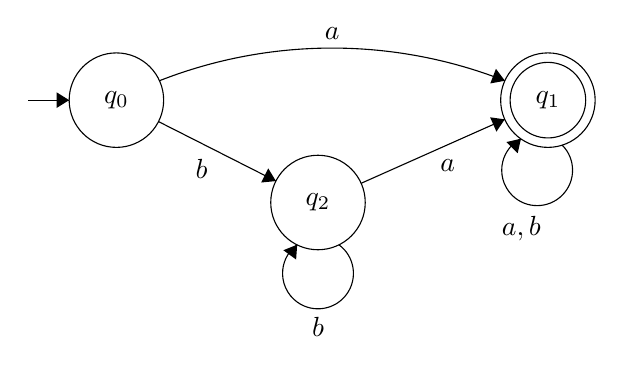
\begin{tikzpicture}[scale=0.2]
\tikzstyle{every node}+=[inner sep=0pt]
\draw [black] (6,-7.8) circle (3);
\draw (6,-7.8) node {$q_0$};
\draw [black] (33.4,-7.8) circle (3);
\draw (33.4,-7.8) node {$q_1$};
\draw [black] (33.4,-7.8) circle (2.4);
\draw [black] (18.8,-14.3) circle (3);
\draw (18.8,-14.3) node {$q_2$};
\draw [black] (8.733,-6.567) arc (111.42324:68.57676:30.025);
\fill [black] (30.67,-6.57) -- (30.1,-5.81) -- (29.74,-6.74);
\draw (19.7,-3.99) node [above] {$a$};
\draw [black] (34.3,-10.65) arc (45.25384:-242.74616:2.25);
\draw (31.71,-15.13) node [below] {$a,b$};
\fill [black] (31.69,-10.25) -- (30.77,-10.46) -- (31.48,-11.17);
\draw [black] (8.67,-9.16) -- (16.13,-12.94);
\fill [black] (16.13,-12.94) -- (15.64,-12.13) -- (15.19,-13.03);
\draw (11.41,-11.55) node [below] {$b$};
\draw [black] (20.123,-16.98) arc (54:-234:2.25);
\draw (18.8,-21.55) node [below] {$b$};
\fill [black] (17.48,-16.98) -- (16.6,-17.33) -- (17.41,-17.92);
\draw [black] (21.54,-13.08) -- (30.66,-9.02);
\fill [black] (30.66,-9.02) -- (29.73,-8.89) -- (30.13,-9.8);
\draw (27.03,-11.56) node [below] {$a$};
\draw [black] (0.4,-7.8) -- (3,-7.8);
\fill [black] (3,-7.8) -- (2.2,-7.3) -- (2.2,-8.3);
\end{tikzpicture}
\end{center}
\end{example}

\begin{exer}
Write out a 5-tuple giving a formal definition for the DFA of Example~\ref{example:fa1}.
\end{exer}

\begin{defn}[DFA Computation]
Let $M = (Q, \Sigma, \delta, q_0, F)$ be a finite automaton and let $w = a_1a_2\cdots a_n$ be a string where each $a_i$ is a member of the alphabet $\Sigma$. Then $M$ \defterm{accepts} $w$ if a sequence of states $r_0, r_1, \ldots, r_n \in Q$ exists with three conditions:
\begin{itemize}
\item $r_0 = q_0$,
\item $\delta(r_i, w_{i+1}) = r_{i+1}$, for $i = 0, \ldots, n-1$, and
\item $r_n \in F$.
\end{itemize}

Informally, an DFA $M$ computes by starting in the start state and then going from state to state, according to its transition function, as it processes symbols from the input string. The machine accepts its input if it ends up in an accept state when it has processed all the symbols in the string.

If $M$ does not accept a string $w$, then we say $M$ \defterm{rejects} $w$.
\end{defn}

\begin{discussion}
When we refer to the finite automata  defined above as being \defterm{deterministic}, we mean that for any state, there is \emph{exactly} one transition that can be taken for each symbol of the alphabet.
\end{discussion}

~

\begin{defn}[Recognizing a language]
We say that $M$ \defterm{recognizes} a language $A$ if $A = \setbuild{w}{M \ \textrm{accepts}\ w}$.
\end{defn}

\begin{exer}
Describe the language recognized by the DFA of Example~\ref{example:fa1}.
\end{exer}

\begin{exer}
Consider the DFA, $M = (\setdef{q_1, q_2}, \setdef{\textrm{0, 1}}, \delta, q_1, \setdef{q_2})$ with transition function $\delta$ given by
\[\begin{array}{c|cc}
 & \textrm{0} & \textrm{1} \\ \hline
 q_1 & q_1 & q_2 \\
 q_2 & q_1 & q_2
\end{array}\]

Draw a state diagram corresponding to the given DFA and describe in a single, concise English sentence the language that it recognizes.
\end{exer}

\begin{defn}[Regular language]
A language is called a \defterm{regular language} if some finite automaton recognizes it.
\end{defn}

\begin{stmt}\label{stmt:dfas}
All of the following languages over the alphabet $\Sigma_{\ref{stmt:dfas}} = \setdef{\texttt{a}, \texttt{b}}$ are regular.
\begin{itemize}
\item $L_1 = \setbuild{w}{\textrm{every \texttt{a} is immediately followed by a \texttt{b}}}$
\item $L_2 = \setbuild{w}{w~\textrm{contains an even number of \texttt{a}'s and an odd number of \texttt{b}'s}}$
\item $L_3 = \setbuild{w}{w~\textrm{contains the substring \texttt{baa}}}$
\item $L_4 = \setbuild{w}{w~\textrm{does not contain the substring \texttt{aab}}}$
\item $L_5 = \setbuild{w}{w~\textrm{has length at least 3 and its third symbol is a}~\texttt{b}}$
\item $L_6 = \setbuild{w}{w~\textrm{starts with \texttt{a} and has odd length, or starts with \texttt{b} and has even length}}$
\item $L_7 = \setbuild{w}{\textrm{every odd position of}~w~\textrm{is an}~\texttt{a}}$
\item $L_8 = \setdef{\emptystring, \texttt{a}}$
\item $L_9 = \emptyset$
\item $L_{10} = $ the set of all strings over $\Sigma_{\ref{stmt:dfas}}$ except the empty string
\end{itemize}
\end{stmt}

\begin{discussion}
Many DFAs contain what is called a \defterm{dead state} or \defterm{error state} -- a non-final state that, once entered, is never exited, no matter what comes later in the input. 
\end{discussion}

\begin{exer}[Vowels in alphabetical order]~\\
Let \[L_\alpha = \setbuild{w \in \setstar{\setdef{\texttt{a} - \texttt{z}}}}{\textrm{all five vowels}\ \texttt{a}, \texttt{e},
			\texttt{i}, \texttt{o}, \texttt{u}, \textrm{occur in alphabetical order in}~w}\]
So $L_\alpha$ contains words like \texttt{abstemious} and \texttt{facetious} but not \texttt{tenacious} or \texttt{tame}. Show that $L_\alpha$ is a regular language.
\end{exer}

\begin{exer}[Floating point numbers]\label{exer:floatingpoint}
~\\Let 
\[L_{\mathrm{float}} = \setbuild{w}{w~\textrm{is the string representation of a floating point number}}\]
Assume the following syntax for floating point numbers:
\begin{itemize}
\item A floating point number is an optional sign, followed by a decimal number, followed by an optional exponent.
\item A decimal number may be of the form $x$ or $x.y$, where $x$ and $y$ are nonempty strings of decimal digits.
\item An exponent beings with \texttt{E} and is followed by an optional sign and then an integer.
\item An integer is a nonempty string of decimal digits.
\end{itemize}
The following strings are examples of floating point numbers:
\[\mathrm{+3.0, 3.0, 0.3E1, 0.3E+1, -0.3E+1, -3E8, 7}\]
Show that $L_{\mathrm{float}}$ is regular.
\end{exer}

% URI language (EAR p61), communication protocol (EAR p62), dispenser (p 55)

\begin{progexer}\happymac
Develop a program that reads in a description of a DFA and then simulates its operation on an input string.
\end{progexer}


\clearpage
\section{Regular Operations}

\begin{discussion}
Since languages are sets, any set operation (union, intersection, difference, complement,\footnote{} etc.) is well-defined on languages. Because languages are sets of strings, there are also some useful operations that we can define on them in terms of those we defined on strings.
\end{discussion}
\footnotetext{For complement, the universal set is considered to be $\setstar\Sigma$ unless otherwise stated.}

\begin{defn}[Regular operations]\label{def:regops}
Let $A$ and $B$ be languages. We define the three \defterm{regular operations} as follows:
\begin{itemize}
\item \defterm{Union}: $\setunion A B = \setbuild{x}{x \in A~\textrm{or}~x \in B}$
\item \defterm{Concatenation}: $\setconcat A B = \setbuild{xy}{x \in A~\textrm{or}~y \in B}$
\item \defterm{Star}: $\setstar A = \setbuild{x_1 x_2 \ldots x_k}{k \geq 0 ~\textrm{and each}~x_i \in A}$
\end{itemize}
\end{defn}

\begin{defn}[Closure]
A set is said to be \defterm{closed} under some operation if applying that operation to any members of the set always produces an object still in the set.
\end{defn}

\begin{thm}
The set of even numbers is \emph{closed under multiplication}.
\end{thm}

\begin{thm}
The set of even numbers is \emph{not closed under division}.
\end{thm}

\begin{exer}
Consider the following languages over the alphabet $\Sigma = \setdef{a, b}$:
\[\begin{array}{l}
L_1 = \setbuild{w}{w~\textrm{contains at least three a's}} \\
L_2 = \setbuild{w}{w~\textrm{contains at least two b's}}
\end{array}\]
Show that each of $L_1$ and $L_2$ is regular and then show that their union, $\setunion{L_1}{L_2}$ is regular.
\end{exer}

\begin{thm}
The set of regular languages is closed under the union operation.
\end{thm}

\begin{exer}
Contemplate whether the set of regular languages is closed under the concatenation operation.
\end{exer}



\clearpage 

\section{Nondeterministic Finite Automata}

\begin{discussion}
Nondeterminism is a concept that is central to the theory of computation. In a deterministic computation, there is always exactly one, unique, way for computation to proceed. In a nondeterministic computation, choices may exist for the next state at any point of the computation. There are a couple of ways to conceptualize nondeterminism. One is to think of all possibilities being explored independently, in parallel. Another is to think of being able to know somehow, as if told by an oracle, which one of the possibilities, if any, will ``work'' when followed and choosing that one.
\end{discussion}

\newcommand\exernfaOne{
\begin{center}
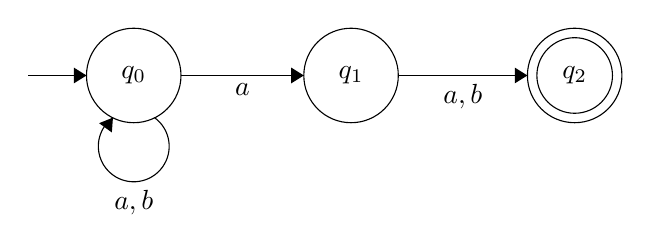
\begin{tikzpicture}[scale=0.2]
\tikzstyle{every node}+=[inner sep=0pt]
\draw [black] (9.7,-7.5) circle (3);
\draw (9.7,-7.5) node {$q_0$};
\draw [black] (23.5,-7.5) circle (3);
\draw (23.5,-7.5) node {$q_1$};
\draw [black] (37.7,-7.5) circle (3);
\draw (37.7,-7.5) node {$q_2$};
\draw [black] (37.7,-7.5) circle (2.4);
\draw [black] (3,-7.5) -- (6.7,-7.5);
\fill [black] (6.7,-7.5) -- (5.9,-7) -- (5.9,-8);
\draw [black] (12.7,-7.5) -- (20.5,-7.5);
\fill [black] (20.5,-7.5) -- (19.7,-7) -- (19.7,-8);
\draw (16.6,-8) node [below] {$a$};
\draw [black] (26.5,-7.5) -- (34.7,-7.5);
\fill [black] (34.7,-7.5) -- (33.9,-7) -- (33.9,-8);
\draw (30.6,-8) node [below] {$a,b$};
\draw [black] (11.023,-10.18) arc (54:-234:2.25);
\draw (9.7,-14.75) node [below] {$a,b$};
\fill [black] (8.38,-10.18) -- (7.5,-10.53) -- (8.31,-11.12);
\end{tikzpicture}
\end{center}}

\begin{exer}\label{exer:nfa1}
The following is a state diagram of a nondeterministic finite automaton (NFA). Identify at least two ways in which it differs from a deterministic finite automaton. Describe the language that it recognizes.
\exernfaOne
\end{exer}

\begin{discussion}
Nondeterministic finite automata may also have arrows labeled $\emptystring$. These allow computation to proceed nondeterministically choosing to either stay at the current state or follow the arrow, without consuming any input. 
\end{discussion}

\begin{exer}
The alphabet of the following nondeterministic finite automaton is simply $\setdef{a}$. Describe the language that is recognized by the NFA.

\begin{center}
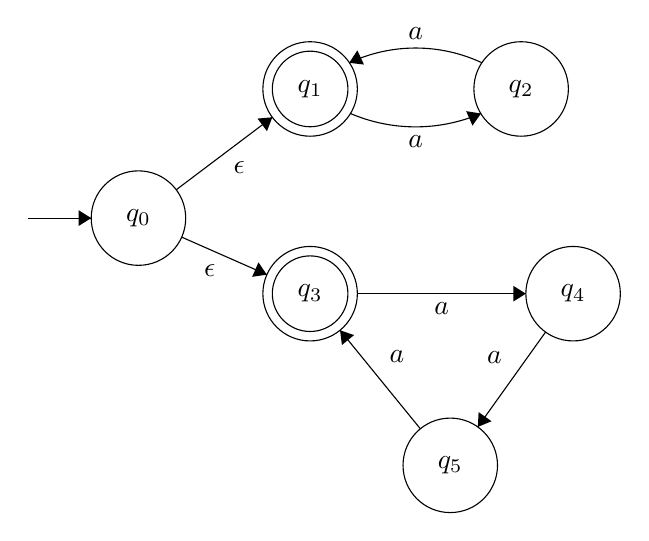
\begin{tikzpicture}[scale=0.2]
\tikzstyle{every node}+=[inner sep=0pt]
\draw [black] (9.6,-18.5) circle (3);
\draw (9.6,-18.5) node {$q_0$};
\draw [black] (20.5,-10.3) circle (3);
\draw (20.5,-10.3) node {$q_1$};
\draw [black] (20.5,-10.3) circle (2.4);
\draw [black] (33.9,-10.3) circle (3);
\draw (33.9,-10.3) node {$q_2$};
\draw [black] (20.5,-23.3) circle (3);
\draw (20.5,-23.3) node {$q_3$};
\draw [black] (20.5,-23.3) circle (2.4);
\draw [black] (37.2,-23.3) circle (3);
\draw (37.2,-23.3) node {$q_4$};
\draw [black] (29.4,-34.2) circle (3);
\draw (29.4,-34.2) node {$q_5$};
\draw [black] (2.6,-18.5) -- (6.6,-18.5);
\fill [black] (6.6,-18.5) -- (5.8,-18) -- (5.8,-19);
\draw [black] (12,-16.7) -- (18.1,-12.1);
\fill [black] (18.1,-12.1) -- (17.16,-12.18) -- (17.76,-12.98);
\draw (16,-14.9) node [below] {$\epsilon$};
\draw [black] (31.347,-11.856) arc (-66.79808:-113.20192:10.526);
\fill [black] (31.35,-11.86) -- (30.41,-11.71) -- (30.81,-12.63);
\draw (27.2,-13.21) node [below] {$a$};
\draw [black] (22.984,-8.639) arc (115.11324:64.88676:9.933);
\fill [black] (22.98,-8.64) -- (23.92,-8.75) -- (23.5,-7.85);
\draw (27.2,-7.2) node [above] {$a$};
\draw [black] (12.35,-19.71) -- (17.75,-22.09);
\fill [black] (17.75,-22.09) -- (17.22,-21.31) -- (16.82,-22.23);
\draw (14.12,-21.41) node [below] {$\epsilon$};
\draw [black] (23.5,-23.3) -- (34.2,-23.3);
\fill [black] (34.2,-23.3) -- (33.4,-22.8) -- (33.4,-23.8);
\draw (28.85,-23.8) node [below] {$a$};
\draw [black] (35.45,-25.74) -- (31.15,-31.76);
\fill [black] (31.15,-31.76) -- (32.02,-31.4) -- (31.2,-30.82);
\draw (32.71,-27.38) node [left] {$a$};
\draw [black] (27.5,-31.88) -- (22.4,-25.62);
\fill [black] (22.4,-25.62) -- (22.52,-26.56) -- (23.29,-25.93);
\draw (25.51,-27.32) node [right] {$a$};
\end{tikzpicture}
\end{center}

\end{exer}

\begin{defn}[$\epsilon$ extension]
For any alphabet $\Sigma$, we write $\Sigma_\epsilon$ to denote $\setunion\Sigma{\setdef{\epsilon}}$.
\end{defn}

\begin{defn}[Nondeterministic finite automaton]
A \defterm{nondeterministic finite automaton} (\defterm{NFA}) is a 5-tuple $(Q, \Sigma, \delta, q_0, F)$ where:
\begin{enumerate}
\item $Q$ is a finite set of states,
\item $\Sigma$ is a finite alphabet,
\item $\delta : \setproduct{Q}{\Sigma_\epsilon} \to \powerset{Q}$ is the transition function,
\item $q_0 \in Q$ is the start state, and
\item $F \subseteq Q$ is the set of accept states.
\end{enumerate}

\end{defn}

\begin{exer}
Describe the domain and range of the transition function of an NFA.
\end{exer}

\begin{exer}
Provide a formal specification for the NFA of Exercise~\ref{exer:nfa1}.
\end{exer}

\begin{defn}[NFA computation]
Let $N = (Q, \Sigma, \delta, q_0, F)$ be an NFA and $w$ be a string over the alphabet $\Sigma$. Then, we say that $N$ \defterm{accepts} $w$ if we can write $w$ as $w = x_1 x_2 \cdots x_n$, where each $x_i \in \Sigma_\epsilon$ and there exists a sequence of states, $r_0, r_1, \ldots, r_n \in Q$ such that:
\begin{enumerate}
\item $r_0 = q_0$,
\item $r_{i+1} \in \delta(r_i, y_{i+1})$,\footnote{Note that $\delta(r_i, y_{i+1})$ is a \emph{set} of possible next states. Contrast the definitions of DFA and NFA.} for $i = 0, \ldots, n-1$, and
\item $r_n \in F$.
\end{enumerate}

As with DFAs, we say that an NFA $N$ \defterm{recognizes} a language $A$ if $A = \setbuild{w}{N~\textrm{accepts}~w}$.
\end{defn}

\begin{exer}
Consider again the language accepted by the following NFA:
\exernfaOne
Determine if it is possible to define a DFA that recognizes the same language.
\end{exer}

\begin{exer}
Describe the language accepted by the following NFA. Then, determine if it is possible to define a DFA that recognizes the same language.
\begin{center}
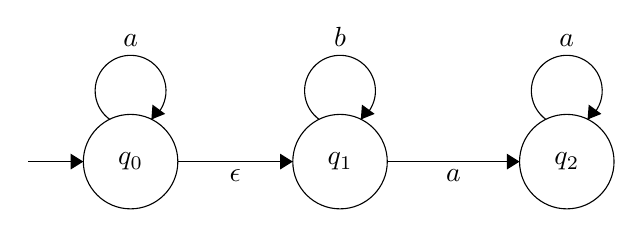
\begin{tikzpicture}[scale=0.2]
\tikzstyle{every node}+=[inner sep=0pt]
\draw [black] (9.3,-10.5) circle (3);
\draw (9.3,-10.5) node {$q_0$};
\draw [black] (22.6,-10.5) circle (3);
\draw (22.6,-10.5) node {$q_1$};
\draw [black] (37,-10.5) circle (3);
\draw (37,-10.5) node {$q_2$};
\draw [black] (2.8,-10.5) -- (6.3,-10.5);
\fill [black] (6.3,-10.5) -- (5.5,-10) -- (5.5,-11);
\draw [black] (12.3,-10.5) -- (19.6,-10.5);
\fill [black] (19.6,-10.5) -- (18.8,-10) -- (18.8,-11);
\draw (15.95,-11) node [below] {$\epsilon$};
\draw [black] (25.6,-10.5) -- (34,-10.5);
\fill [black] (34,-10.5) -- (33.2,-10) -- (33.2,-11);
\draw (29.8,-11) node [below] {$a$};
\draw [black] (7.977,-7.82) arc (234:-54:2.25);
\draw (9.3,-3.25) node [above] {$a$};
\fill [black] (10.62,-7.82) -- (11.5,-7.47) -- (10.69,-6.88);
\draw [black] (21.277,-7.82) arc (234:-54:2.25);
\draw (22.6,-3.25) node [above] {$b$};
\fill [black] (23.92,-7.82) -- (24.8,-7.47) -- (23.99,-6.88);
\draw [black] (35.677,-7.82) arc (234:-54:2.25);
\draw (37,-3.25) node [above] {$a$};
\fill [black] (38.32,-7.82) -- (39.2,-7.47) -- (38.39,-6.88);
\end{tikzpicture}
\end{center}
\end{exer}

\begin{progexer}\happymac
Develop a program that reads in a description of an NFA and produces a description of an equivalent DFA.
\end{progexer}

\begin{progexer}\happymac
Develop a program that reads in a description of an NFA and then simulates its operation on an input string.
\end{progexer}


\begin{thm}
Every nondeterministic finite automaton has an equivalent deterministic finite automaton.\footnote{}
\end{thm}\footnotetext{For the purposes of this course, it will be sufficient for you to show a construction that is reasonably convincing and intuitively correct. Time permitting, we go over a proof of its correctness together in class.}

\begin{corol}
A language is regular if and only if some nondeterministic finite automaton recognizes it.
\end{corol}

\begin{exer}
Convert the following NFAs to equivalent DFAs.

\begin{tabular}{c@{\ \ \ \ \ \ \ \ \ \ \ \ \ }c}
\\
(a) & (b) \\
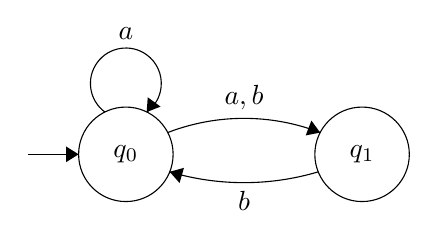
\begin{tikzpicture}[scale=0.2]
\tikzstyle{every node}+=[inner sep=0pt]
\draw [black] (8.5,-10.6) circle (3);
\draw (8.5,-10.6) node {$q_0$};
\draw [black] (23.5,-10.6) circle (3);
\draw (23.5,-10.6) node {$q_1$};
\draw [black] (2.3,-10.6) -- (5.5,-10.6);
\fill [black] (5.5,-10.6) -- (4.7,-10.1) -- (4.7,-11.1);
\draw [black] (7.177,-7.92) arc (234:-54:2.25);
\draw (8.5,-3.35) node [above] {$a$};
\fill [black] (9.82,-7.92) -- (10.7,-7.57) -- (9.89,-6.98);
\draw [black] (11.156,-9.218) arc (111.0991:68.9009:13.457);
\fill [black] (20.84,-9.22) -- (20.28,-8.46) -- (19.92,-9.4);
\draw (16,-7.82) node [above] {$a,b$};
\draw [black] (20.718,-11.712) arc (-73.41019:-106.58981:16.525);
\fill [black] (11.28,-11.71) -- (11.91,-12.42) -- (12.19,-11.46);
\draw (16,-12.9) node [below] {$b$};
\end{tikzpicture}

&
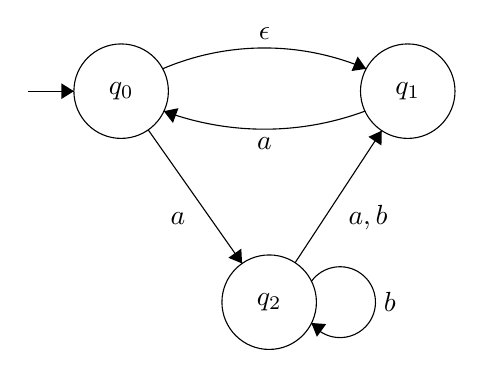
\begin{tikzpicture}[scale=0.2]
\tikzstyle{every node}+=[inner sep=0pt]
\draw [black] (9.9,-9.8) circle (3);
\draw (9.9,-9.8) node {$q_0$};
\draw [black] (28.1,-9.8) circle (3);
\draw (28.1,-9.8) node {$q_1$};
\draw [black] (19.3,-23.2) circle (3);
\draw (19.3,-23.2) node {$q_2$};
\draw [black] (4,-9.8) -- (6.9,-9.8);
\fill [black] (6.9,-9.8) -- (6.1,-9.3) -- (6.1,-10.3);
\draw [black] (12.537,-8.378) arc (113.11693:66.88307:16.462);
\fill [black] (25.46,-8.38) -- (24.92,-7.6) -- (24.53,-8.52);
\draw (19,-6.56) node [above] {$\epsilon$};
\draw [black] (25.385,-11.068) arc (-69.64162:-110.35838:18.353);
\fill [black] (12.61,-11.07) -- (13.19,-11.82) -- (13.54,-10.88);
\draw (19,-12.71) node [below] {$a$};
\draw [black] (11.62,-12.26) -- (17.58,-20.74);
\fill [black] (17.58,-20.74) -- (17.53,-19.8) -- (16.71,-20.38);
\draw (14,-17.86) node [left] {$a$};
\draw [black] (21.98,-21.877) arc (144:-144:2.25);
\draw (26.55,-23.2) node [right] {$b$};
\fill [black] (21.98,-24.52) -- (22.33,-25.4) -- (22.92,-24.59);
\draw [black] (20.95,-20.69) -- (26.45,-12.31);
\fill [black] (26.45,-12.31) -- (25.6,-12.7) -- (26.43,-13.25);
\draw (24.31,-17.83) node [right] {$a,b$};
\end{tikzpicture}
\end{tabular}

\end{exer}

\begin{discussion}
You may have already proved the following theorem. Try proving it again, using the notion of an NFA that we have now defined. 
\end{discussion}

\begin{thm}
The set of regular languages is closed under the union operation.
\end{thm}

\begin{thm}
The set of regular languages is closed under the concatenation operation.
\end{thm}

\begin{thm}
The set of regular languages is closed under the star operation.
\end{thm}

\begin{corol}
The set of regular languages is closed under the regular operations (Definition~\ref{def:regops}).
\end{corol}

\newcommand\charA{{\texttt{a}}}
\newcommand\charB{{\texttt{b}}}

\begin{stmt}\label{stmt:nfas}
All of the following languages are regular.
\begin{itemize}
\item $L_1 = \setbuild{\charA^n\charB\charA^m}{n, m \geq 0, n \equiv_3 m}$
\item $L_2 = \setbuild{w\in\setstar{\setdef{0-9}}}{
\parbox{4in}{$w$~corresponds to the decimal encoding of a natural number whose encoding contains, as a substring,
			the encoding of a natural number that is divisible by 3}
			}$
\item $L_3 = \setbuild{w\in\setstar{\setdef{\charA, \charB, \texttt{c}}}}{|w| \geq 2\ \textrm{and}\ w\ \textrm{begins and ends with the same symbol}}$


%\item $L_1 = \setbuild{w}{\textrm{every \texttt{a} is immediately followed by a \texttt{b}}}$
%\item $L_2 = \setbuild{w}{w~\textrm{contains an even number of \texttt{a}'s and an odd number of \texttt{b}'s}}$
%\item $L_3 = \setbuild{w}{w~\textrm{contains the substring \texttt{baa}}}$
%\item $L_4 = \setbuild{w}{w~\textrm{does not contain the substring \texttt{aab}}}$
%\item $L_5 = \setbuild{w}{w~\textrm{has length at least 3 and its third symbol is a}~\texttt{b}}$
%\item $L_6 = \setbuild{w}{w~\textrm{starts with \texttt{a} and has odd length, or starts with \texttt{b} and has even length}}$
%\item $L_7 = \setbuild{w}{\textrm{every odd position of}~w~\textrm{is an}~\texttt{a}}$
%\item $L_8 = \setdef{\emptystring, \texttt{a}}$
%\item $L_9 = \emptyset$
%\item $L_{10} = $ the set of all strings over $\Sigma_{\ref{stmt:dfas}}$ except the empty string
\end{itemize}
\end{stmt}




\section{Regular Expressions}\label{sec:regexp}


\begin{defn}[Regular expression]
Given an alphabet $\Sigma$, a \defterm{regular expression}, $R$, is defined as one of:
\begin{enumerate}
\item $\emptyset$,
\item $\emptystring$,
\item $a$ for some $a \in \Sigma$,
\item $(R_1 + R_2)$, where $R_1$ and $R_2$ are regular expressions,
\item $(R_1 \cdot R_2)$, where $R_1$ and $R_2$ are regular expressions,
\item ${R_1}^*$, where $R_1$ is a regular expression.
\end{enumerate}

For convenience, we may omit parentheses in an expression, in which case the order of precedence of the latter three operators is: $*$, then $\cdot$, then $+$.\footnote{i.e. $(R_1 + {R_2}^* \cdot R_3) = (R_1 + (({R_2}^*) \cdot R_3))$ } Also, for convenience, we write $R^+$ for $R^*$, $R^k$ for the concatenation of $k$ $R$'s with each other, and $R_1 R_2$ (omitting the dot) for $R_1 \cdot R_2$.
\end{defn}

\begin{discussion}
The purpose of regular expressions is to describe a language exclusively by means of single symbols from the alphabet, the special symbols $\emptyset, \emptystring, \union, \circ, *$, and parentheses.
\end{discussion}

\begin{defn}[Language of a regular expression]
The language represented by a regular expression, $R$, written as $\langof R$, is defined as:
\begin{enumerate}
\item $\langof\emptyset = \emptyset$.
\item $\langof\emptystring = \setdef\emptystring$.
\item $\langof{a} = \setdef{a}$ for any $a \in \Sigma$.
\item $\langof{R_1 + R_2} = \setunion{\langof{R_1}}{\langof{R_2}}$
\item $\langof{R_1 \cdot R_2} = {\langof{R_1}}\circ{\langof{R_2}}$
\item $\langof{R^*} = \left(\langof{R}\right)^*$
\end{enumerate}
Note, the latter three map regular expressions, on the left, to regular operations on languages, on the right.
\end{defn}

\begin{exer}
For each regular expression that follows, describe the language it represents as concisely as possible. Assume the language is $\Sigma = \setdef{0, 1}$. Note that we use the shorthand of $\Sigma$ inside a regular expression to represent $(0 + 1)$.
\begin{enumerate}
\item $0^*10^*$
\item $\Sigma^*1\Sigma^*$
\item $\Sigma^*001\Sigma^*$
\item $1^*(01^+)^*$
\item $(\Sigma\Sigma\Sigma)^*$
\item $01 + 10$
\item $0 + 1 + 0\Sigma^*0 + 1\Sigma^*1$
\item $(0 + \emptystring)(1 + \emptystring)$
\item $1^*\emptyset$
\item $\emptyset^*$
\end{enumerate}
\end{exer}

\begin{exer}
Write a regular expression that represents the language 
\[\setbuild{w\in\setstar{\setdef{a, b}}}{w~\textrm{contains an odd number of $a$'s}}.\]
\end{exer}

\begin{exer}
~\\Let $L_{\mathrm{float}}$ be defined as in Exercise~\ref{exer:floatingpoint}:
\[L_{\mathrm{float}} = \setbuild{w}{w~\textrm{is the string representation of a floating point number}}\]
Let $D = \setdef{0, 1, 2, 3, 4, 5, 6, 7, 8, 9}$. Write a regular expression, $R$, such that $\langof R = L_{\mathrm{float}}$.
\end{exer}

\begin{lemma}
If a language is described by a regular expression, then there exists an NFA that recognizes the same language.
\end{lemma}

\begin{discussion}
For the next lemma that you prove, consider introducing a generalized type of nondeterministic finite automaton (GNFA) in which the arrows are labeled with regular expressions (instead of single symbols). Given a DFA, it should be straightforward to convert it to such a GNFA with the additional properties that it has one single start state that has no incoming arrows, one single accept state that has no outgoing arrows, and one arrow going from every state to every other state including the state itself. Then, show how such a GNFA with $n$ number of states can be shrunk down to an equivalent GNFA with only two states (the start and accept states) and a single arrow between them, labeled with a regular expression.

\noindent For example, the following portion of such an automaton:
\begin{center}
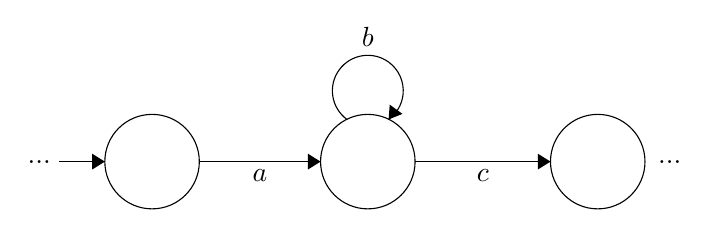
\begin{tikzpicture}[scale=0.2]
\tikzstyle{every node}+=[inner sep=0pt]
\draw [black] (9.9,-9.8) circle (3);
\draw [black] (23.6,-9.8) circle (3);
\draw [black] (38.2,-9.8) circle (3);
\draw (42,-9.8) node [right] {$...$};
\draw [black] (4,-9.8) -- (6.9,-9.8);
\draw (3.5,-9.8) node [left] {$...$};
\fill [black] (6.9,-9.8) -- (6.1,-9.3) -- (6.1,-10.3);
\draw [black] (12.9,-9.8) -- (20.6,-9.8);
\fill [black] (20.6,-9.8) -- (19.8,-9.3) -- (19.8,-10.3);
\draw (16.75,-10.3) node [below] {$a$};
\draw [black] (22.277,-7.12) arc (234:-54:2.25);
\draw (23.6,-2.55) node [above] {$b$};
\fill [black] (24.92,-7.12) -- (25.8,-6.77) -- (24.99,-6.18);
\draw [black] (26.6,-9.8) -- (35.2,-9.8);
\fill [black] (35.2,-9.8) -- (34.4,-9.3) -- (34.4,-10.3);
\draw (30.9,-10.3) node [below] {$c$};
\end{tikzpicture}
\end{center}
might be simplified in one step to:
\begin{center}
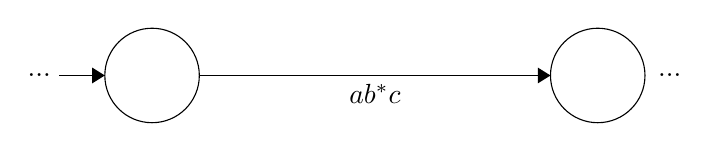
\begin{tikzpicture}[scale=0.2]
\tikzstyle{every node}+=[inner sep=0pt]
\draw [black] (9.9,-9.8) circle (3);
\draw [black] (38.2,-9.8) circle (3);
\draw (42,-9.8) node [right] {$...$};
\draw [black] (4,-9.8) -- (6.9,-9.8);
\draw (3.5,-9.8) node [left] {$...$};
\fill [black] (6.9,-9.8) -- (6.1,-9.3) -- (6.1,-10.3);
\draw [black] (12.9,-9.8) -- (35.2,-9.8);
\fill [black] (35.2,-9.8) -- (34.4,-9.3) -- (34.4,-10.3);
\draw (24.05,-10.3) node [below] {$ab^*c$};
\end{tikzpicture}
\end{center}

\end{discussion}

\begin{lemma}
If a language is recognized by a DFA, then there exists a regular expression that represents the same language.
\end{lemma}

\begin{thm}
A language is regular if and only if some regular expression describes it.
\end{thm}

\clearpage

\section{Regular and Non-regular Languages}

\begin{discussion}
Are there languages that are not regular?
\end{discussion}

% can talk about countably infinite # of reg languages, but uncountably infinite number of languages on non-empty alphabet - so more languages than regular languages

\begin{thm}
Every finite language is regular.
\end{thm}

\begin{defn}[Reverse of a language]
For any language $A$, let $\stringrev{A} = \setbuild{\stringrev{w}}{w \in A}$. 
\end{defn}

\begin{thm}
If $A$ is a regular language, so is $\stringrev{A}$.
\end{thm}

\begin{exer}
Let
\[
\Sigma_3 = \left\{ \left[\begin{array}{c}0\\0\\0\end{array}\right],
			   \left[\begin{array}{c}0\\0\\1\end{array}\right],
			  \left[\begin{array}{c}0\\1\\0\end{array}\right],
		          \cdots,
		          \left[\begin{array}{c}1\\1\\1\end{array}\right]
		  \right\}
\]
$\Sigma_3$ contains all size 3 columns of 0s and 1s. A string of symbols in $\Sigma_3$ may be read as three rows of 0s and 1s. Consider each row to be a binary number and let
\[
B = \setbuild{w\in\setstar{\Sigma_3}}{\textrm{the bottom row of $w$ is the sum of the top two rows}}.
\]

For example,
\[
\left[\begin{array}{c}0\\0\\1\end{array}\right]
\left[\begin{array}{c}1\\0\\0\end{array}\right]
\left[\begin{array}{c}1\\1\\0\end{array}\right]
\in B, \quad \quad \textrm{but} \quad \quad
\left[\begin{array}{c}0\\0\\1\end{array}\right]
\left[\begin{array}{c}1\\0\\1\end{array}\right]
\notin B.
\]
Show that $B$ is regular. 
\hint Working with $\stringrev B$ is easier.
\end{exer}

\begin{discussion}
The preceding exercise shows that DFAs are powerful enough to recognize (i.e. \emph{compute}) binary addition.
\end{discussion}

\begin{thm}
Let $B_n = \setbuild{\charA^k}{k~\textrm{is a multiple of}~n}$. For every $n \geq 1$, the language $B_n$ is regular.
\end{thm}

\begin{exer}
Let $D = \setbuild{\charA^n \charB^n}{n \geq 0}$. Formulate a statement regarding the regularity of the language $D$ and prove it.
\end{exer}

\begin{discussion}
We now prove a general theorem that is true for every regular language. This theorem will not be particularly useful if we already know a language is regular, and it won't help us show that a particular language \emph{is} regular if we don't already know. However, it can be very useful for constructing proofs by contradiction to show that a particular language \emph{is not} regular.
\end{discussion}

\begin{lemma}
Let $M = (Q, \Sigma, \delta, q_0, F)$ be a DFA. If $M$ accepts any string of length $|Q|$ or greater, then that string must force $M$ to visit some state in $Q$ more than once (thus traversing at least one loop).
\end{lemma}

\begin{thm}[Pumping lemma for regular languages]
If $A$ is a regular language, then there exists a number $p$ (called the \defterm{pumping length}) such that if $s$ is any string in $A$ of length at least $p$, then $s$ can be divided into three pieces, $s = xyz$, satisfying the following conditions:
\begin{enumerate}
\item $xy^iz \in A$ for all $i \geq 0$,
\item $|y| > 0$,\footnote{} and
\item $|xy| \leq p$.
\end{enumerate}
\end{thm}\footnotetext{i.e. $y \neq \emptystring$.}

\begin{discussion}
Use the pumping lemma to prove the following by contradiction.
\end{discussion}

\begin{thm}
Let $D = \setbuild{\charA^n \charB^n}{n \geq 0}$. $D$ is not regular.
\end{thm}

\begin{thm}
Let $E = \setbuild{w \in \setstar{\setdef{\charA, \charB}}}{w~\textrm{has an equal number of \charA{s} and \charB{s}}}$. $E$ is not regular.
\end{thm}

\begin{thm}
Let $G = \setbuild{\charA^n \charB^m}{n > m}$. $G$ is not regular.
\end{thm}

\begin{thm}
Let $BP = \setbuild{w \in \setstar{\setdef{), (}}}{\textrm{the parentheses are balanced}}$. $BP$ is not regular.
\end{thm}


\begin{thm}
Let $P = \setbuild{w\stringrev{w}}{w \in \setstar{\setdef{\charA, \charB}}}$. $P$ is not regular.
\end{thm}

\begin{thm}
Let $O = \setbuild{\charA^{n^2}}{n \geq 0}$. $O$ is not regular.
\end{thm}


\vspace{.3in}
\hrule 
\vspace{.3in}

\begin{discussion}
After completing a body of work, it is satisfying and helpful to put together the ideas in your mind -- to see the forest beyond the trees. Take some time to do that by considering the following questions.
\end{discussion}

\begin{exer}
So far, we have explored several formalisms used to describe languages. How are they related? How are they different? Are there aspects that are somewhat surprising? What are their computational abilities and limitations? Type up a page with your \emph{thoughtful} reflections.
\end{exer}



%%%%%%%%%%%%%%%%%%%%%%%%%%%%%%
\chapter{Context-Free Languages}


%%%%%%%%%%%%%%%%%%%%%%%%%%%%%%
\part{Computability}


%%%%%%%%%%%%%%%%%%%%%%%%%%%%%%
\part{Complexity}



% TODO
% cardinality of sets - lewis pg 20 (sec 1.4)


%\part{}
%\chapter{}
%\section{}
%\subsection{}
%\subsubsection{}
%\paragraph{}
%\subparagraph{}



\end{document}  